	\chapter{Results and discussion}

The survey of Andromeda Galaxy according to \cite{observed} gives us the rotation curve measured out to $38$ kpc, showing a peak at $340$ km s$^{-1}$, a dip at $202$ km s$^{-1}$ around $4$ kpc, two distinct flat parts at $264$ km s$^{-1}$  and $230$ km s$^{-1}$ and an increase to $275$  km s $^{-1}$ in the outermost regions \cite{observed}.
\begin{figure} [h]
\centering
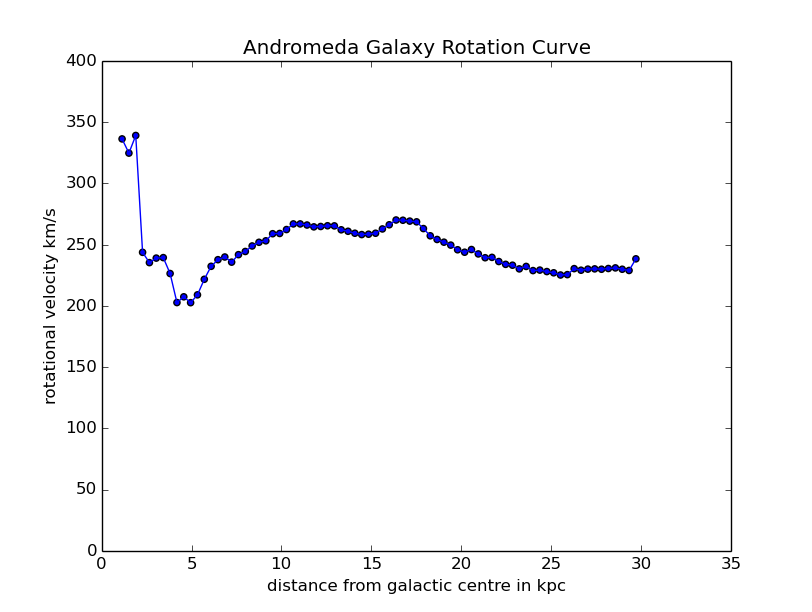
\includegraphics[scale=0.5]{rotcurve}
\caption{Observed Rotation Curve for Andromeda Galaxy}
\end{figure}

\section{Optimized Rotation Curve}

The rotation curve obtained from the data, that was calculated using Image Analysis as explained in section $ 2.2.1 $ was optimized, and the resulting plot is:

\begin{figure} [h]
\centering
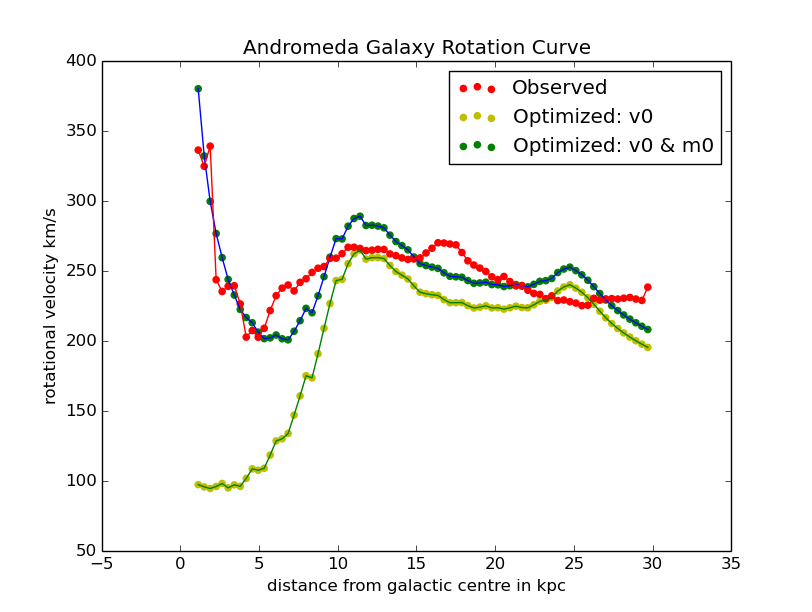
\includegraphics[scale=0.5]{best}
\caption{Rotation Curve for Andromeda Galaxy}
\label{curves}
\end{figure}

\section{Need for Optimization}

The rotation curve obtained by using the precalculated data, was to be achieved by the data calculated using image analysis. When we plotted the curve from our calculated data, it gave us an irregular pattern, which demanded that some fitting be done. After we optimized the graph to a certain velocity the optimization function gave us the fitted value of $v_0$ . From Figure \ref{curves} we found the curve described as \textit{optimized for velocity} \textbf{$v_{0}$} to be somewhat in accordance with the observed rotation curve, but it still required significant modification in the region near the origin.
To that end we optimized the curve for central mass and consequently the function gave us optimized value of \textbf{$m_{0}$}. 

The values of $v_{0}$ and $m_{0}$ were calculated to be;

$v_{0} = 55802.2453 $         

$m_{0} = 1473818.3329 $

with standard deviations of:

$\triangle v =  683.96$

$\triangle m = 88311.38 $

$v_0$ being a scaling factor is dimensionless while $m_0$ is measured in the same arbitrary units as the masses calculated using image analysis. To make sense of $m_0$ note that it is $16$ percent of the total calculated mass of the galaxy.